\section{TextSeal 2: Confidence smoothing
(adapted)}\label{record-docs-watermarking-qualitative-text-textseal2-smoothing-md-textseal-2-confidence-smoothing-adapted}

This is a fresh answer to the same prompt, not a rewrite.

Eight pairs selected by fixed test positions before inspecting detection
or quality outcomes. Undetected originals and unsuccessful attacks
remain included.

\begin{recordfigure}
\centering
\pandocbounded{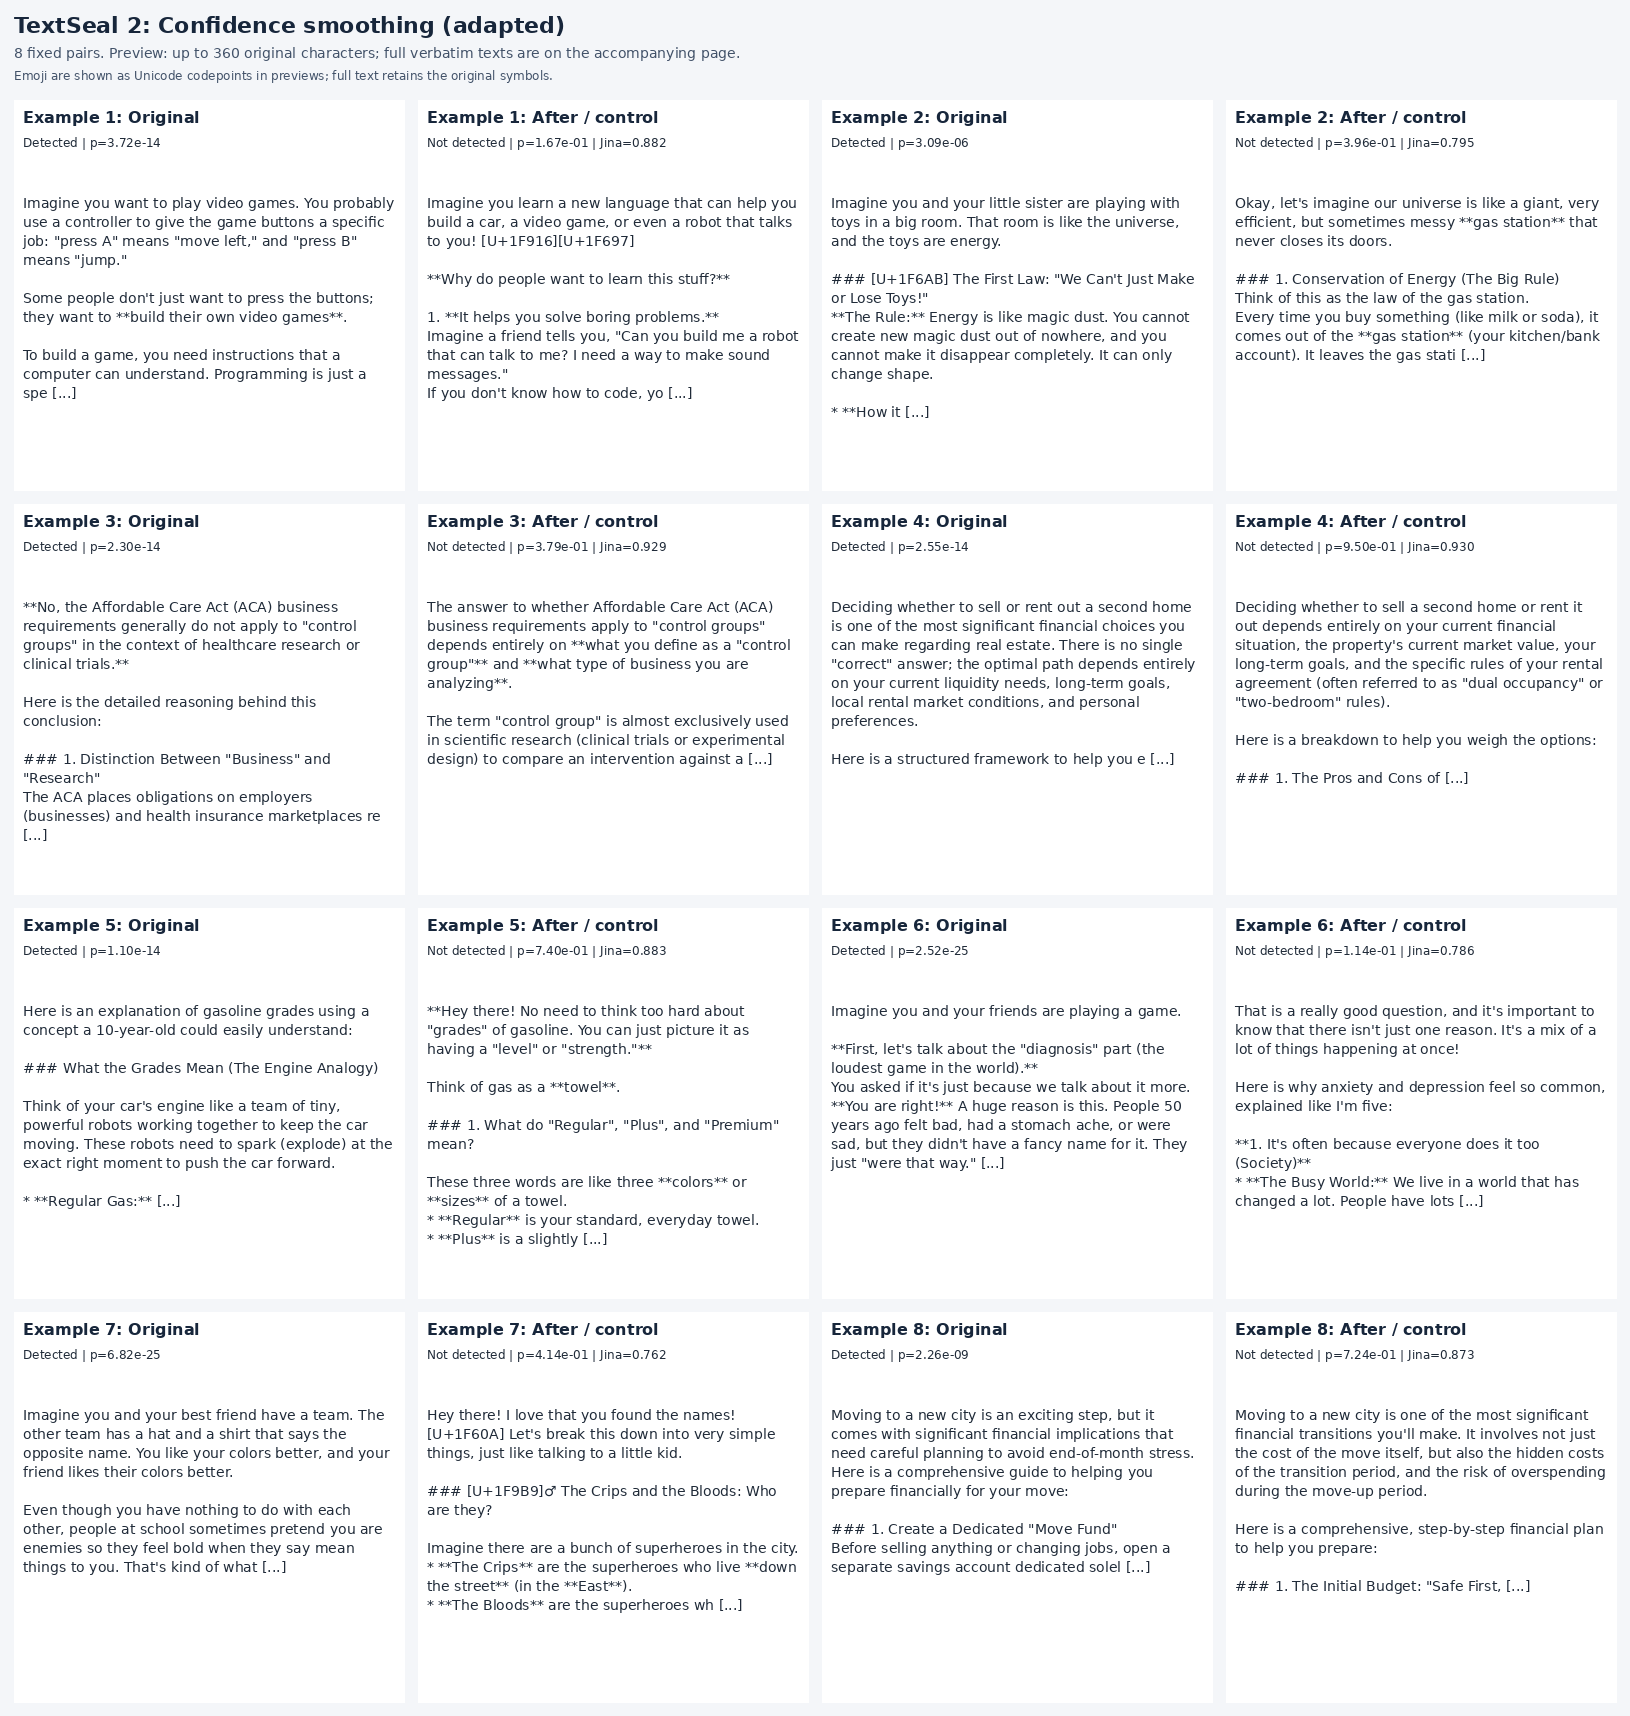
\includegraphics[keepaspectratio,alt={Sixteen-panel text preview}]{figures/text-textseal2-smoothing.png}}
\caption{Sixteen-panel text preview}
\end{recordfigure}

The figure previews up to the first 360 original characters per
response; full texts below are unabridged. Emoji use Unicode codepoints
in the preview to avoid missing-glyph boxes. Owner scores and quality
metrics use full responses.

{\scriptsize\setlength{\tabcolsep}{3pt}\def\LTcaptype{none} % do not increment counter
\begin{longtable}[]{@{}
  >{\raggedright\arraybackslash}p{(\linewidth - 8\tabcolsep) * \real{0.2000}}
  >{\raggedright\arraybackslash}p{(\linewidth - 8\tabcolsep) * \real{0.2000}}
  >{\raggedright\arraybackslash}p{(\linewidth - 8\tabcolsep) * \real{0.2000}}
  >{\raggedright\arraybackslash}p{(\linewidth - 8\tabcolsep) * \real{0.2000}}
  >{\raggedright\arraybackslash}p{(\linewidth - 8\tabcolsep) * \real{0.2000}}@{}}
\toprule\noalign{}
\begin{minipage}[b]{\linewidth}\raggedright
Example
\end{minipage} & \begin{minipage}[b]{\linewidth}\raggedright
Test position
\end{minipage} & \begin{minipage}[b]{\linewidth}\raggedright
Before
\end{minipage} & \begin{minipage}[b]{\linewidth}\raggedright
After
\end{minipage} & \begin{minipage}[b]{\linewidth}\raggedright
Jina
\end{minipage} \\
\midrule\noalign{}
\endhead
\bottomrule\noalign{}
\endlastfoot
1 & 0 & Detected \textbar{} p=3.72e-14 & Not detected \textbar{}
p=1.67e-01 & 0.8821 \\
2 & 32 & Detected \textbar{} p=3.09e-06 & Not detected \textbar{}
p=3.96e-01 & 0.7950 \\
3 & 64 & Detected \textbar{} p=2.30e-14 & Not detected \textbar{}
p=3.79e-01 & 0.9292 \\
4 & 96 & Detected \textbar{} p=2.55e-14 & Not detected \textbar{}
p=9.50e-01 & 0.9301 \\
5 & 128 & Detected \textbar{} p=1.10e-14 & Not detected \textbar{}
p=7.40e-01 & 0.8833 \\
6 & 160 & Detected \textbar{} p=2.52e-25 & Not detected \textbar{}
p=1.14e-01 & 0.7858 \\
7 & 192 & Detected \textbar{} p=6.82e-25 & Not detected \textbar{}
p=4.14e-01 & 0.7623 \\
8 & 224 & Detected \textbar{} p=2.26e-09 & Not detected \textbar{}
p=7.24e-01 & 0.8731 \\
\end{longtable}
}

\subsection{Example 1: test position
0}\label{record-docs-watermarking-qualitative-text-textseal2-smoothing-md-example-1-test-position-0}

Prompt ID:
\texttt{\seqsplit{eb41610306c3726e0a74a6888b55bc82ea505683f3fe908e286b197665852b84}}.

\textbf{Question / prompt}

\begin{Verbatim}
Why do people want programming taught in elementary / high schools ? I know absolutely nothing about programming . EDIT : I 'm marking this as answered . Thanks to everyone who replied ! Explain like I'm five.
\end{Verbatim}

\textbf{Original watermarked-model output}

\begin{Verbatim}
Imagine you want to play video games. You probably use a controller to give the game buttons a specific job: "press A" means "move left," and "press B" means "jump."

Some people don't just want to press the buttons; they want to **build their own video games**.

To build a game, you need instructions that a computer can understand. Programming is just a special language that tells the computer what to do. It's like writing the "rulebook" for the computer to follow.

People teach this to kids because:
1.  **It's a superpower:** Just like learning to speak English helps you talk to friends, learning code helps you talk to computers.
2.  **It builds good habits:** Programming teaches kids to be very patient (computers don't have feelings!) and to solve puzzles step-by-step, just like solving a math problem.
3.  **It changes how the world works:** Soon, they
\end{Verbatim}

\textbf{After / alternative output}

\begin{Verbatim}
Imagine you learn a new language that can help you build a car, a video game, or even a robot that talks to you! [U+1F916][U+1F697]

**Why do people want to learn this stuff?**

1.  **It helps you solve boring problems.**
    Imagine a friend tells you, "Can you build me a robot that can talk to me? I need a way to make sound messages."
    If you don't know how to code, you have to ask the whole school to make a robot. But if you learn programming, you can write the simple rules (like "make this sound like a beep!") and tell the robot to do it.

2.  **It makes things easier to do.**
    If your teacher says, "This class is about how to make things move," and you just learn *why* things move, you won't know how to make a video game. But if you learn how to write the code
\end{Verbatim}

Recorded diagnostics:
\texttt{\seqsplit{\{"mistral\_perplexity": 7.5\}}}.

\subsection{Example 2: test position
32}\label{record-docs-watermarking-qualitative-text-textseal2-smoothing-md-example-2-test-position-32}

Prompt ID:
\texttt{\seqsplit{55ce85cdcf38f9b189c667d07ffb34cc5bd73600e98a2987c721e3a8c166c343}}.

\textbf{Question / prompt}

\begin{Verbatim}
Thermodynamics Could someone explain to me the first , and second laws of thermodynamics , and conservation of energy ? Explain like I'm five.
\end{Verbatim}

\textbf{Original watermarked-model output}

\begin{Verbatim}
Imagine you and your little sister are playing with toys in a big room. That room is like the universe, and the toys are energy.

### [U+1F6AB] The First Law: "We Can't Just Make or Lose Toys!"
**The Rule:** Energy is like magic dust. You cannot create new magic dust out of nowhere, and you cannot make it disappear completely. It can only change shape.

*   **How it works:** If you blow up a balloon, you used energy from your breath to make the rubber stretch. If that balloon pops, the energy doesn't vanish; it turns into a tiny *whoosh* of sound and a little bit of heat warming up the room.
*   **The Secret:** The total amount of toys in the whole room stays exactly the same forever. Energy just changes clothes (from movement to heat, from heat to light), but the total number never goes up or down.

### [U+1F504] The Second Law: "The Toys
\end{Verbatim}

\textbf{After / alternative output}

\begin{Verbatim}
Okay, let's imagine our universe is like a giant, very efficient, but sometimes messy **gas station** that never closes its doors.

### 1. Conservation of Energy (The Big Rule)
Think of this as the law of the gas station.
Every time you buy something (like milk or soda), it comes out of the **gas station** (your kitchen/bank account). It leaves the gas station and gets put back in your account (your wallet/pouch).

**The Rule:**
Energy is like gold or electricity. You can never take it out of the gas station and make it disappear. You also can't make it disappear out of the gas station.
*   If you have money (**Energy**), and you spend it on a snack, the snack leaves the money.
*   The money stays in the gas station (in bank accounts).
*   If you sell the snack, you take the money out of the snack (gas station)
\end{Verbatim}

Recorded diagnostics:
\texttt{\seqsplit{\{"mistral\_perplexity": 9.3125\}}}.

\subsection{Example 3: test position
64}\label{record-docs-watermarking-qualitative-text-textseal2-smoothing-md-example-3-test-position-64}

Prompt ID:
\texttt{\seqsplit{3cd335e45281f1d50700d93f931fc20b2f8fef24b7084ab3b583f745105137b1}}.

\textbf{Question / prompt}

\begin{Verbatim}
Do Affordable Care Act business requirements apply to “control groups?”
\end{Verbatim}

\textbf{Original watermarked-model output}

\begin{Verbatim}
**No, the Affordable Care Act (ACA) business requirements generally do not apply to "control groups" in the context of healthcare research or clinical trials.**

Here is the detailed reasoning behind this conclusion:

### 1. Distinction Between "Business" and "Research"
The ACA places obligations on employers (businesses) and health insurance marketplaces regarding health coverage mandates, minimum essential coverage (MEC), and marketplaces. These are statutory requirements designed to regulate the market and prevent bare minimum coverage scenarios.

"Control groups," however, are a fundamental concept in **clinical research, epidemiology, and data science**. They are cohorts of individuals used in scientific studies to compare the effects of an intervention (treatment) against a baseline to establish causality. They are not inherently "business entities" (like an employer or insurance carrier) subject to ACA compliance rules regarding hiring, insurance purchasing, or marketplace enrollment.

### 2. Specific Contexts Where ACA Might Interfere
\end{Verbatim}

\textbf{After / alternative output}

\begin{Verbatim}
The answer to whether Affordable Care Act (ACA) business requirements apply to "control groups" depends entirely on **what you define as a "control group"** and **what type of business you are analyzing**.

The term "control group" is almost exclusively used in scientific research (clinical trials or experimental design) to compare an intervention against a baseline. It is **not** a standard industry term for a specific business unit, division, or market segment in the context of regulatory compliance.

Here is the logical breakdown:

### 1. If You Are Conducting Research (Scientific/Experimental Context)
If you are conducting a clinical trial or a market research study with a specific focus on a subset of businesses (the "control group"), you are applying scientific methodology, not business rules.
*   **Mechanism:** In a controlled experiment, the control group consists of businesses that do not receive the marketing, sales, or regulatory intervention, while the intervention group does.
*  
\end{Verbatim}

Recorded diagnostics:
\texttt{\seqsplit{\{"mistral\_perplexity": 8.75\}}}.

\subsection{Example 4: test position
96}\label{record-docs-watermarking-qualitative-text-textseal2-smoothing-md-example-4-test-position-96}

Prompt ID:
\texttt{\seqsplit{28bb030845669613f0466940878780ef6fe5149ef4223cb7b87d0ce22e4d30b3}}.

\textbf{Question / prompt}

\begin{Verbatim}
Should I sell a 2nd home, or rent it out?
\end{Verbatim}

\textbf{Original watermarked-model output}

\begin{Verbatim}
Deciding whether to sell or rent out a second home is one of the most significant financial choices you can make regarding real estate. There is no single "correct" answer; the optimal path depends entirely on your current liquidity needs, long-term goals, local rental market conditions, and personal preferences.

Here is a structured framework to help you evaluate both options.

### 1. The Case for SELLING
Selling the property is generally the better choice if you are looking for **immediate cash flow**, wish to **minimize maintenance**, or plan to **convert existing equity into liquid assets**.

*   **Liquidity and Equity:** You turn a "sick chicken" (non-performing asset) into immediate cash. This is ideal if you have high mortgage interest payments that drag down your overall portfolio's return.
*   **Cost Efficiency:** Maintenance, taxes, insurance, and repairs can drain $500–$2,000+ annually for
\end{Verbatim}

\textbf{After / alternative output}

\begin{Verbatim}
Deciding whether to sell a second home or rent it out depends entirely on your current financial situation, the property's current market value, your long-term goals, and the specific rules of your rental agreement (often referred to as "dual occupancy" or "two-bedroom" rules).

Here is a breakdown to help you weigh the options:

### 1. The Pros and Cons of Selling
**Why you might sell:**
*   **Immediate Cash Injection:** Selling converts your investment into liquid cash, which you can use for living expenses, paying off debts, or buying new property elsewhere.
*   **Clear Title:** If you have an existing rental mortgage, selling clears the title, allowing you to refinance the entire property or start a new mortgage.
*   **Time and Maintenance:** Selling removes the daily stress of repairs, cleaning, tenant issues, and inventory management. You are off the hook for those responsibilities.
*   **Tax Benefits (for some):** Depending
\end{Verbatim}

Recorded diagnostics:
\texttt{\seqsplit{\{"mistral\_perplexity": 6.84375\}}}.

\subsection{Example 5: test position
128}\label{record-docs-watermarking-qualitative-text-textseal2-smoothing-md-example-5-test-position-128}

Prompt ID:
\texttt{\seqsplit{ba7280e98e1cd80ce7a2ecb56c06dcc0cccae5126f2c806c9c87951a5c32a351}}.

\textbf{Question / prompt}

\begin{Verbatim}
Can somebody explain what different grades of gasoline mean ( regular , plus , premium ) and why I should use anything but regular ? Edit : Thanks guys , despite getting up to 10 year old vocabulary , you 've answered my question very well Explain like I'm five.
\end{Verbatim}

\textbf{Original watermarked-model output}

\begin{Verbatim}
Here is an explanation of gasoline grades using a concept a 10-year-old could easily understand:

### What the Grades Mean (The Engine Analogy)

Think of your car's engine like a team of tiny, powerful robots working together to keep the car moving. These robots need to spark (explode) at the exact right moment to push the car forward.

*   **Regular Gas:** This is the standard "All-Stars" version. Most cars were designed to run on this. The robots in your engine are strong enough to do their job with the spark coming from the regular gas.
*   **Midgrade (Plus):** This is like "All-Stars and a Backup." It has a little bit more power added to the mix, meaning the explosion happens slightly earlier and with a bit more force. Some older cars or slightly faster ones use this, but it's not strictly necessary for average drivers.
*   **Premium Gas:** This is the "Pro Team
\end{Verbatim}

\textbf{After / alternative output}

\begin{Verbatim}
**Hey there! No need to think too hard about "grades" of gasoline. You can just picture it as having a "level" or "strength."**

Think of gas as a **towel**.

### 1. What do "Regular", "Plus", and "Premium" mean?

These three words are like three **colors** or **sizes** of a towel.
*   **Regular** is your standard, everyday towel.
*   **Plus** is a slightly bigger towel (so it gets a little easier to wipe away).
*   **Premium** is the giant, super strong towel that covers a whole lot.

Here is the rule: **More gas = stronger towel!**
If you want a very strong towel to wipe away oil or dirt, you should buy the **Premium** one. If you just want a small towel for a spot, a **Regular** one is fine.

### 2. Why should you use anything
\end{Verbatim}

Recorded diagnostics:
\texttt{\seqsplit{\{"mistral\_perplexity": 7.15625\}}}.

\subsection{Example 6: test position
160}\label{record-docs-watermarking-qualitative-text-textseal2-smoothing-md-example-6-test-position-160}

Prompt ID:
\texttt{\seqsplit{b1f1f19f49ef99f6892eb93dd82a9582e1819ca3b02645f3d8eb75d6851036e9}}.

\textbf{Question / prompt}

\begin{Verbatim}
Howcome anxiety and depression are so common ? Is it something to do with society and lifestyles or how children are raised ? Or is it simply because it 's more acceptable to talk about it which means it 's more easily diagnosed ? Explain like I'm five.
\end{Verbatim}

\textbf{Original watermarked-model output}

\begin{Verbatim}
Imagine you and your friends are playing a game.

**First, let's talk about the "diagnosis" part (the loudest game in the world).**
You asked if it's just because we talk about it more. **You are right!** A huge reason is this. People 50 years ago felt bad, had a stomach ache, or were sad, but they didn't have a fancy name for it. They just "were that way." Today, we know exactly what to look for! Doctors have a special list of words to describe these feelings. So, if someone feels a little sad now, they can easily say, "I have depression!" Because we use the word so much, we find these feelings in more people than we used to. It's like realizing that almost everyone has a crush on a favorite cartoon character[U+2014]you didn't know it existed as a super-power before!

**Next, let's look at the "how we live" part (the
\end{Verbatim}

\textbf{After / alternative output}

\begin{Verbatim}
That is a really good question, and it's important to know that there isn't just one reason. It's a mix of a lot of things happening at once!

Here is why anxiety and depression feel so common, explained like I'm five:

**1. It's often because everyone does it too (Society)**
*   **The Busy World:** We live in a world that has changed a lot. People have lots of homework, work, and games to play all day. It's easy to feel sad or worried when the world isn't going right with us.
*   **The "Big Bad Wolf":** There is this scary story called "The Big Bad Wolf" in the stories. It says the wolf is a scary scary thing. In our world, there are scary things too, like bad news, bad grades, or even a bad teacher. When a scary thing happens, it's easy to feel sad or scared.

**2. Why it
\end{Verbatim}

Recorded diagnostics:
\texttt{\seqsplit{\{"mistral\_perplexity": 8.75\}}}.

\subsection{Example 7: test position
192}\label{record-docs-watermarking-qualitative-text-textseal2-smoothing-md-example-7-test-position-192}

Prompt ID:
\texttt{\seqsplit{413d7314d50fdc47803344b8bf0b0e9291797c0b2e2296b73b1d78a212e69257}}.

\textbf{Question / prompt}

\begin{Verbatim}
What is the difference between the Crips and the Bloods . Why are they rivals ? What do each do ? Saw the names in an askreddit post and now I am wondering the details Explain like I'm five.
\end{Verbatim}

\textbf{Original watermarked-model output}

\begin{Verbatim}
Imagine you and your best friend have a team. The other team has a hat and a shirt that says the opposite name. You like your colors better, and your friend likes their colors better.

Even though you have nothing to do with each other, people at school sometimes pretend you are enemies so they feel bold when they say mean things to you. That's kind of what happened with two groups of friends in a big city named **The Crips** and **The Bloods**.

Here is the difference, what they do, and why they are rivals, explained simply:

### 1. Why are they rivals?
They aren't fighting because one team lost a video game or because one group of people stole candy. There was no "cheating" to stop them from being mean to each other.

It started long ago when black and Latino teenagers in Los Angeles got into a small fight. Later, people in different parts of the city started forming their own groups based on
\end{Verbatim}

\textbf{After / alternative output}

\begin{Verbatim}
Hey there! I love that you found the names! [U+1F60A] Let's break this down into very simple things, just like talking to a little kid.

### [U+1F9B9][U+200D][U+2642][U+FE0F] The Crips and the Bloods: Who are they?

Imagine there are a bunch of superheroes in the city.
*   **The Crips** are the superheroes who live **down the street** (in the **East**).
*   **The Bloods** are the superheroes who live **right next door** (in the **West**).

You remember the movies or news stories? That was when they fought! Now they are just two friends playing together.

### [U+2694][U+FE0F] Why are they rivals? (The Story)

They are rivals because they used to fight for power. Before today, there was only one gang fighting. The main boss wanted to be the only superhero and win the title of "Superhero King."

One of the C
\end{Verbatim}

Recorded diagnostics:
\texttt{\seqsplit{\{"mistral\_perplexity": 8.25\}}}.

\subsection{Example 8: test position
224}\label{record-docs-watermarking-qualitative-text-textseal2-smoothing-md-example-8-test-position-224}

Prompt ID:
\texttt{\seqsplit{3bca8fb40ea23a3b89f55baf6f1df768cadc687ae8a97bbbfc98c7db825a44ac}}.

\textbf{Question / prompt}

\begin{Verbatim}
I am moving to a new city. How do I plan and prepare - financially - for the move?
\end{Verbatim}

\textbf{Original watermarked-model output}

\begin{Verbatim}
Moving to a new city is an exciting step, but it comes with significant financial implications that need careful planning to avoid end-of-month stress. Here is a comprehensive guide to helping you prepare financially for your move:

### 1. Create a Dedicated "Move Fund"
Before selling anything or changing jobs, open a separate savings account dedicated solely to moving costs.
*   **Set a timeline:** Aim to have 3–6 months of rent (in the new city) plus the full moving budget saved up before you pack.
*   **Budget categories:** Break down your expected costs into:
    *   **Housing Deposits:** Typically 1–2 months' rent upfront.
    *   **Security Deposits:** Often $500–$2,000 depending on the city and damage guarantees.
    *   **Moving Services/Packing:** Truck rental, professional movers, or self-move supplies.
    *   **Utilities & First
\end{Verbatim}

\textbf{After / alternative output}

\begin{Verbatim}
Moving to a new city is one of the most significant financial transitions you'll make. It involves not just the cost of the move itself, but also the hidden costs of the transition period, and the risk of overspending during the move-up period.

Here is a comprehensive, step-by-step financial plan to help you prepare:

### 1. The Initial Budget: "Safe First, Then Safe Second"
The most common mistake is starting the move with a full budget. You need to establish a **safe, conservative budget** first to ensure you have enough money for the essentials.

*   **Step 1: Define your baseline.** Calculate what you can afford to spend on essentials in the new city without feeling guilty.
*   **Step 2: Set a "Buffer."** Once you have that baseline, add an extra 10–20% contingency fund just for unexpected costs (e.g., unexpected medical bills, local service fees, or lost items).
\end{Verbatim}

Recorded diagnostics:
\texttt{\seqsplit{\{"mistral\_perplexity": 7.875\}}}.

\href{records/docs/watermarking/text.tex}{Text metrics} \textbar{}
\href{../docs/watermarking/README.md}{Report overview}
